\chapter{Background}
\label{chaBackground}
A sufficient basis to understand this work is presented in this chapter.

% Programming languages in general is considered one of the more mature topics in computer science. There are many, many books and papers written on compilers. Some programmers even consider compilers to be black boxes which they must obey, frightened of the complexities and details of the black magic working inside. This background aims to unbox these beasts called compilers and shed some light on them. Explaining all the details of a compiler and the type checker is out of scope for this background.
% 
% Wordlengths, HDLs and also get a section describing how they fit into this work.


\section{Introduction to Compiler Structure}
What constitutes a compiler is not always obvious. A compiler, in the most banal sense, takes an input program and outputs an output program. Some want the output to be ``simpler`` than the input, passing in a high level program in C and outputting executable X86 machine code where X86 is considered a ``simpler`` than C. The input to the compiler is often text, and we will assume this for the rest of this short introduction to compilers.

Each compiler is unique, but they often have a shared structure. The first step is often to do lexical analysis (also called lexing) in a lexer or tokenizer. Here characters are abstracted away, and the compiler has done the first processing of the text. When lexing you often decide what piece of text is an integer-constant, a keyword, a string, etc. After the lexing the tokens are used to perform semantic analysis -- parsing. During parsing the compiler understands structures in the program such as what is part of each function or correctly parsing the order of operations for mathematical expressions. The parsing usually produces an abstract syntax tree (AST). Though some compilers interweave these steps, they are usually there in spirit.

The Spade compiler has both a lexer step and a parser step which are located in different modules.

The compilers work is not done yet. After all the syntactical analysis the semantic analysis can be started, semantic analysis is sometimes referred to as the ``inner layers of the compiler``. Here we resolve identifiers, run type-checking and other static program analysis or do optimizations like moving around constants to avoid needless copies. The wordlength inference and optimizations will be an inner layer, the relevant details will be discussed in the Section \ref{sec:TypeChecking}. 

After the compiler has finished optimizing, the output is generated and potentially lowered (made less complex) in multiple stages, often by translating to a simpler internal representation which in the end makes generating the final output of the compiler easier.

One ``layer`` is often called a ``pass``. Spade is not a multi-pass compiler and perform these steps sequentially -- not interleaved.
\cite{src:DragonBook}\cite{src:CraftingInterp}\cite{src:KKLectures}

\begin{figure}
\begin{center}
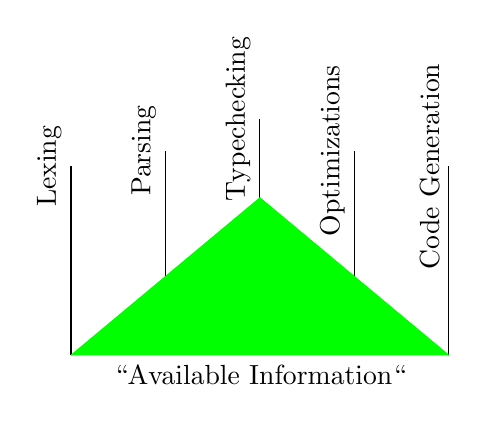
\begin{tikzpicture}[xscale=3, yscale=2]
% vertical lines
\draw (0,0) -- (0,1.2) node[above, rotate=90] {Lexing};
\draw (0.4,0) -- (0.4,1.3) node[above, rotate=90] {Parsing};
\draw (0.8,0) -- (0.8,1.5) node[above, rotate=90] {Typechecking};
\draw (1.2,0) -- (1.2,1.3) node[above, rotate=90] {Optimizations};
\draw (1.6,0) -- (1.6,1.2) node[above, rotate=90] {Code Generation};
% horizontal line
\filldraw[color=green, fill=green] (0,0) -- (0.8,1.0) -- (1.6,0);
\draw (0.8,0.0) node[below] {``Available Information``};
\end{tikzpicture}
  \caption{A visualization of the rough measurement of information present in each step of the compilation process. Typechecking having the most information and lexing and code generation having the least amount of information.}
  \label{fig:InformationCompilation}
\end{center}
\end{figure}

Compilers have to construct a lot of complex information about the program. A visual some find helpful when reasoning about compilers is an imagined graph of ``available information``. Figure \ref{fig:InformationCompilation} tries to communicate the amount of information created in each step of compilation. The most important part being that we know a lot about the program in the type checking phase.

\todo{monomorphisation}

\section{Type Checking} % Maybe `inner layers`?
\label{sec:TypeChecking}
Type checking is a way of making sure the program is internally consistent, there are no contradictions inside to program to the program itself. Type checking can be done in different ways with different pros, cons or preferences \cite{src:TypeCheckersBook}. The type checker in Spade can infer types and deduce things about the program, like ``the first argument is a 3-bit integer value, but you gave a record`` \cite{src:spadeAnHDL}. Typechecking has shown to reduce some kinds of programming errors and can in some cases even suggest what functions to use.

The type checker in Spade is a one directional Damas–Hindley–Milner type checker. This means it stops on the first error and can deduce types to their most general form. So if asked to type check the identity function (a function that takes one value and returns the value as is, the function does nothing) the type checker would be able to deduce that the argument could have any type, but that the type is the same as the return value, without any help from the programmer except the body of the function. \cite{src:DamasHindleyMilner}

There is also a connected topic of type inference -- a program that guesses the types of expressions based on the context. A sufficiently good typeinferrer could be used to check the types of the program and can easily be modded into a typechecker. It is infact upon this idea that the Damas–Hindley–Milner typechecker works. In this paper, we will freely refer to typecheckers and work by typeinferrence as both typecheckers and typeinferrence -- even though it might not be the most correct according to the literature we deem it adds variety and clarity to how these systemms function.

\subsection{Unification}
\todo{Fill this in!}

\section{Interval Arithmetic, Affine Arithmetic and Self Validating Numerical Methods}
\label{sec:IAndAA}

There is an excellent explanation of both Interval- and Affine Arithmetic by \citeauthor{src:affAri} -- the following section is a short version to cover the absolute basics of the material.

Affine arithmetic and interval arithmetic and two common ways to estimate. They can be applied to estimate bounds for mathematical functions or things that can be modeled by mathematical functions. They also have a place in static analysis of programs, which is the focuses of this thesis. This section describes what these concepts are, references literature if you want to read more and shows their roll in static analysis of programs. These methods are often referred to as over-estimation.

\todo{Motivate why we chose to only use AA and IA}
Though affine arithmetic is more sophisticated it does not always produce better results, interval arithmetic can for some computations produce tighter bounds. There are other methods for overestimation that are considered more sophisticated like ME-gPC and modified affine arithmetic, but the extra complexity can be added later if it is found to be needed \cite{src:MEgPC}. For motivations of why are not considered see section \ref{sec:MotivationIAndAA}.

\subsection{Interval Arithmetic}
Interval arithmetic operates on intervals, as the name implies. A value -- or in the context of a program, a variable -- has a smallest and largest value it can assume. Consider \verb`x = random_real()`, where \verb`random_real` generates a random value in the range $[0, 1]$. We can express this in interval arithmetic as $\bar{x} = [0, 1]$, intervals will be denoted with a bar on top to separate them from the variables. Note especially that the true value of $x$ lies in the interval $\bar{x}$. In this example we know $0 \leq x \leq 1$, also written as $x \in [0, 1]$. These intervals can be added, negated, and so on, to give you an estimate of an arbitrary expression.

For a more throughout guide on implementations \citetitle{src:affAri} by \citeauthor{src:affAri} is worth your time, this section will cover the basics that are needed to understand the concept and understand this thesis. A full description of the field is out of scope.

\subsubsection{Interval Arithmetic Special values}
When doing static program analysis, some extra values are often defined. For example, it is okay to have an interval where one value is infinite. This interval $[5, \infty]$ is perfectly valid.

The empty interval is also defined and written as $[]$. The empty interval usually denotes expressions or code that cannot be reached or evaluated. It might seem useless at a glance, but is required to do more sophisticated static analysis.
\Todo{IA, have shorter definitions written in ``affine-and-interval-arithmetic.md``, maybe just refer to the original sources since it is not really relevant except for the implementation, unless we get a specific result due to one of them.}

\subsubsection{Interval Arithmetic: An example and Limitations}
Examples are often helpful.
We will be using the expression $2x + z - z$ as an example where $x = [0, 1], z = [1, 3]$.

\begin{verbatim}
2 * [0, 1] + [1, 3] - [1, 3]
// Scaling rule and subtraction is negated addition 
[2 * 0, 2 * 1] + [1, 3] + (-1 * [1, 3])
// Calculate
[0, 2] + [1, 3] + [-3, -1]
// Sum it upp
[-2, 4]
\end{verbatim}

This gives us the conclusion that this expression will lie in the range $[-2, 4]$ for the given values of $x$ and $z$. This is true, but the estimate is larger than it necessarily needs to be. An observant reader would notice that subtracting the value $z$ from itself should result in $0$, which is a perfectly valid point. This is a limitation of the interval arithmetic. Interval arithmetic does not reason about the expressions that came before it and how they combine, and this limitation would exist if used to do static analysis of programs. This limitation leads us to affine arithmetic which understands the relations between variables we evaluate. Affine arithmetic can more accurately calculate expressions like $a - a$ since it understands that $a$ and $a$ is the same thing.


\subsection{Affine Arithmetic}
Affine arithmetic (AA) works similarly to interval arithmetic (IA), but has a memory of where values come from and can reason about their combinations at a higher level. That said, AA does not produce strictly better results than IA in all circumstances and a combination is currently thought to be the current state of the art. 

\subsubsection{How Affine Arithmetic works}
In affine arithmetic there is a concept of noise symbols ($e_i$ where $i$ is a natural number) and the numbers half width ($x_i$ where $i$ is a natural number). A linear combination of these noise symbols is a reasonable way to represent a "number" when reasoning about affine arithmetic, $\hat{x} = x_0 + x_1e_1 + x_2e_2 + \dots$. These terms can them be combined using similar rules to interval arithmetic.

Notice how the first term lacks a noise symbol, this expresses where the center of the uncertainty is. The different noise variables serve as the memory of this expression, consider subtracting $\hat{x} - \hat{x}$ with itself we get the expected result of 0 from that.

\Todo{Something about how multiplication works}

\subsection{Error Explosion for Affine- and Interval Arithmetic}
Both affine arithmetic and interval arithmetic compensate for unknown factors with a span of potential values. This method is fine for most computations that are small and simple, but this isn't always the case. Some calculations result in large spans of potential values -- since a smaller span gives more certainty and are easier to account for.

For the use case of circuits and FPGAs which are relevant for Spade this can be a large problem. This problem is further discussed in section \ref{sec:MotivationIAndAA}.

\Todo{Don't know how good this is}

\cite{src:affAri}

\section{Wordlength Inference and Typechecking in Spade}
\label{sec:TheProblem}
Most values in Spade take up bits or space in the run time environment. Wordlength inference is mostly concerned with numbers -- so consider positive numbers without a decimal. Consider a program with a counter that resets to 0 after counting to 3, we do not need 32 bits to represent it. The cost of storing a number with 32 bits compared to 2 bits could be large if it requires a larger FPGA, extra circuit components or a different power rating. Compared to software where memory is considered abundant -- this causes Spade as a HDL to be designed differently compared to a highlevel programming language.

Wordlength inference is the compiler understanding what wordlength -- the number of bits -- is needed to store a value. Inferring this value well causes good resource usage and requires less manual intervention. Doing it poorly or not at all either requires users to manually specify the wordlength of each value, or a hardware that is inefficient.

\begin{figure}[h]
\begin{center}
\begin{verbatim}
fn f(a: int<3>) -> int<4> {
  a + 1 + 1
}

entity main(clk: clock, rst: bool) -> int<4> {
  f(3)
}
\end{verbatim}
\end{center}
\label{fig:SimpleFaultSpade}
\caption{``simple\_fault.spade`` A simple spade program that does not compile, showing the current limitations of wordlength inference.}
\end{figure}

\begin{figure}[h]
\begin{center}
\begin{verbatim}
error: Type error
  ┌─ src/simple\_fault.spade:1:27
  │
1 │   fn f(a: int<3>) -> int<4> {
  │                      ------ int<4> type specified here
  │ ╭───────────────────────────^
2 │ │   a + 1 + 1
3 │ │ }
  │ ╰─^ Found type int<5>
  │
  = Expected: 4
  =       in: int<4>
  =      Got: 5
  =       in: int<5>

Error: aborting due to previous error
\end{verbatim}
\end{center}
\label{fig:SimpleFaultSpadeCompileOutput}
\caption{The output from the compiler when trying to compile the program ``simple\_fault.spade``}
\end{figure}

Consider the program in Figure \ref{fig:SimpleFaultSpade}. The function ``f`` adds 3 values together, two of which are known constants. We also know that $2^3 + 2 < 2^4$ -- we should be able to fit the result of the addition into the 4 bit word without loss of data. The compiler does not agree as seen in the compiler output in Figure \ref{fig:SimpleFaultSpadeCompileOutput} where it claims we need 5 bits to store this value. This problem might seem inconsequential since calculating constant expressions during compilation would fix this, as seen by the program in Figure \ref{fig:SimpleCorrectSpade} compiling without worries. Only fixing this problem for constants would be nice variables would cause the same problem to appear but in a more difficult form. The problem here is much deeper, and is a direct cause of the typechecking algorithm itself.

\begin{figure}[h]
\begin{center}
\begin{verbatim}
fn f(a: int<3>) -> int<4> {
  a + 2
}

entity main(clk: clock, rst: bool) -> int<4> {
  f(3)
}
Error: aborting due to previous error
\end{verbatim}
\end{center}
\label{fig:SimpleCorrectSpade}
\caption{``simple\_correct.spade`` A spade program that does compile, which is very similar to the program in Figure \ref{fig:SimpleFaultSpade}}
\end{figure}

\todo{Maybe change to using screen shoots? But I like the idea of it being text since it's usually easier to read... Hmm...}
\todo{Move this to the typechecking section?}
The Spade compiler implements a the Damas-Hindley–Milner type checker -- a fast and modern type checker for simple type systems. Damas-Hindley-Milner runs in almost linear time (if implemented correctly) but is not complete. The completeness property for type checkers means there are programs which are correct but that the type checker will not recognize as correct. The programs from Figures \ref{fig:SimpleFaultSpade} and \ref{fig:SimpleCorrectSpade} are an example of this. This observation is important since it means this is not a bug, but a limitation of the compiler itself. How this should be changed and to what is the central topic of this thesis.

\section{Spade}
Spade is a HDL taking a lot of inspiration from Rust to create a more modern HDL (Hardware Description Language). Spade has syntax which mimics that of Rust and tries to remove problems people have when using other HDLs like System Verilog. One of the biggest features of Spade is the static typechecking which allows programs to be verified before even being synthesised -- creating a faster iteration loop.
\cite{src:spadeSomething} \cite{src:spadeAnHDL}

% \section{FPGA}
\Todo{Explain what an FPGA is and what makes it different from micro controllers}

\Todo{I need to explain Swim}


%%%%%%%%%%%%%%%%%%%%%%%%%%%%%%%%%%%%%%%%%%%%%%%%%
% Related Work
%%%%%%%%%%%%%%%%%%%%%%%%%%%%%%%%%%%%%%%%%%%%%%%%%

\chapter{Related Work}
\Todo{Needs a lot more content here, and it is a very well studied subject}

\section{Minimization of Fractional Wordlength on Fixed-Point Conversion for High-Level Synthesis}
Minimization of Fractional Wordlength on Fixed-Point Conversion for High-Level Synthesis suggests a method for using as few bits in the fractional part of values as possible. Their approach resulted in decent optimizations and was much faster than doing the optimization by hand. The sample size of the programs is quite small and did not always show as promising results.

\cite{src:MinOfFrac}

\section{High-level synthesis and arithmetic optimizations}
The thesis ``High-level synthesis and arithmetic optimizations`` is an attempt to merge the fields of arithmetic with and HDL-compilers. Several approaches are evaluated that affect correctness, throughput and latency. It describes fixed-point and floating point arithmetic, FPGA hardware and FPGA optimizations in a very clear way.

Problems with the IEEE floating point numbers are mentioned, for one how the implicit rounding causes addition to be non-associative, and how C/C++ compilers used for HDL use CPU optimizations which are not always suitable for FPGA.

\citeauthor{src:HLSandOpt} is an alternative approach to Spade when it comes to generating hardware and it tries to generate better FPGA hardware by modifying a compilation layer for the current compilers. But C/C++ has a fundamental problem when being mapped to hardware, the languages were built for single-threaded sequential computations where FPGAs prefer to do computations in parallel.

\cite{src:HLSandOpt}

\Todo{Software development methods}



% # Planned literature supporting the thesis
% - Books and papers on IA and AA
%   - Self-Validated Numerical Methods and Applications
% - Static analysis books and literature, potentially digging into bounded model checking (BMC) and the likes
%   - Calculus of Computation, maybe more literature here
% - The course on program analysis available on LiU 
%   - TDDE34 and the presentations there
% - Previous literature on Spade
%   - Spade: An HDL Inspired by Modern Software Languages and co
% - Books and papers on type checkers and compilers books and literature
%   - Some papers on Henk are interesting
%   - Complete and Easy Bidirectional Typechecking for Higher-Rank Polymorphism
%   - Types and Programming Languages by Ben Pierce
% - There is a lot of FPGA literature on FPGA optimization, here are a few
%    - Constantinides, George A.
%      Word-length Optimization for Differentiable Nonlinear Systems
%    - N. Doi and T. Horiyama and M. Nakanishi and S. Kimura
%      Minimization of fractional wordlength on fixed-point conversion for high-level synthesis
%    - Have like 10 more of these...

